% Fig. 2 (method). PAGE width (7.1 in = 18.03 cm). Compile: pdflatex method.tex
% Colours follow paper/scripts/figures/style.py: source and start = GRAY, target and student = SLOT[0],
% teacher and weak labels = SLOT[6], text = INK / INK2.
\documentclass[tikz,border=1pt]{standalone}
\usepackage[T1]{fontenc}
\usepackage[scaled]{helvet}
\renewcommand{\familydefault}{\sfdefault}
\usepackage{amsmath}
\usepackage{sfmath}
\usepackage[none]{hyphenat}
\usetikzlibrary{arrows.meta,positioning,calc,shapes.geometric}
\definecolor{src}{HTML}{8A8985}
\definecolor{tgt}{HTML}{2A78D6}
\definecolor{tea}{HTML}{6250D6}
\definecolor{ink}{HTML}{0B0B0B}
\definecolor{ink2}{HTML}{52514E}
\tikzset{
  >={Stealth[length=4pt,width=3.4pt]},
  every node/.style={font=\scriptsize, text=ink},
  box/.style={draw, rounded corners=2pt, line width=0.6pt, align=left, inner sep=3.5pt, fill=white, anchor=north west},
  flow/.style={->, line width=0.8pt, draw=ink2},
  db/.style={cylinder, shape border rotate=90, aspect=0.25, line width=0.5pt, minimum width=0.95cm, minimum height=0.62cm},
  lab/.style={fill=tgt, draw=white, line width=0.3pt},
}
\begin{document}
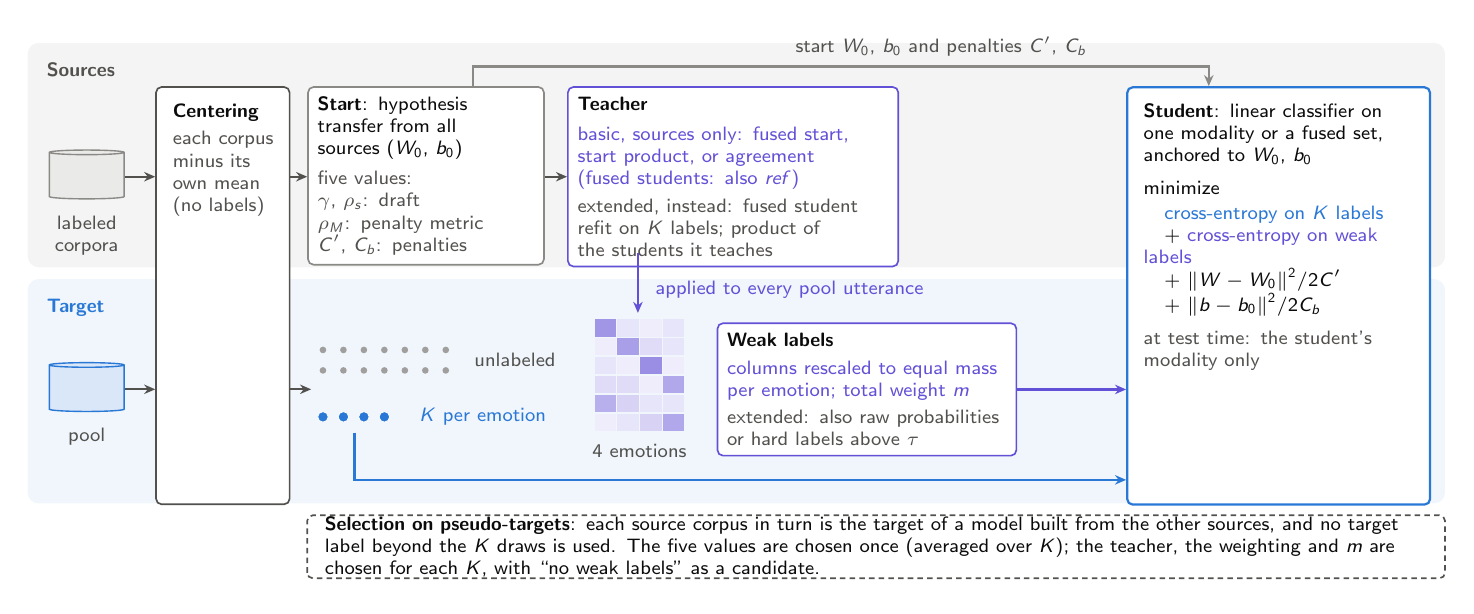
\begin{tikzpicture}
% ------------------------------------------------------------------ lanes
\fill[src!9, rounded corners=4pt] (0,4.0) rectangle (18.0,6.85);
\fill[tgt!7, rounded corners=4pt] (0,1.0) rectangle (18.0,3.85);
\node[anchor=north west, font=\scriptsize\bfseries, text=ink2] at (0.12,6.72) {Sources};
\node[anchor=north west, font=\scriptsize\bfseries, text=tgt] at (0.12,3.72) {Target};

% ------------------------------------------------------------------ data
\node[db, draw=src, fill=src!18] (sdb) at (0.75,5.15) {};
\node[anchor=north, align=center, text=ink2] at (0.75,4.78) {labeled\\corpora};
\node[db, draw=tgt, fill=tgt!18] (tdb) at (0.75,2.45) {};
\node[anchor=north, align=center, text=ink2] at (0.75,2.08) {pool};

% ------------------------------------------------------------------ centering (both lanes)
\node[box, draw=ink2, text width=1.45cm, minimum height=5.3cm] (cen) at (1.62,6.3) {};
\node[anchor=north west, align=left, text width=1.45cm] at (1.72,6.2)
  {\textbf{Centering}\\[2pt]\textcolor{ink2}{each corpus}\\\textcolor{ink2}{minus its}\\\textcolor{ink2}{own mean}\\\textcolor{ink2}{(no labels)}};
\draw[flow] (sdb.east) -- (sdb.east -| cen.west);
\draw[flow] (tdb.east) -- (tdb.east -| cen.west);

% ------------------------------------------------------------------ start
\node[box, draw=src, text width=2.75cm] (start) at (3.55,6.3)
  {\textbf{Start}: hypothesis\\transfer from all\\sources ($W_0$, $b_0$)\\[3pt]
   \textcolor{ink2}{five values:}\\
   \textcolor{ink2}{$\gamma$, $\rho_s$: draft}\\
   \textcolor{ink2}{$\rho_M$: penalty metric}\\
   \textcolor{ink2}{$C'$, $C_b$: penalties}};
\draw[flow] (cen.east |- 0,5.15) -- (start.west |- 0,5.15);

% ------------------------------------------------------------------ teacher
\node[box, draw=tea, text width=3.95cm] (teach) at (6.85,6.3)
  {\textbf{Teacher}\\[3pt]
   \textcolor{tea}{basic, sources only: fused start,}\\
   \textcolor{tea}{start product, or agreement}\\
   \textcolor{tea}{(fused students: also \emph{ref})}\\[2pt]
   \textcolor{ink2}{extended, instead: fused student}\\
   \textcolor{ink2}{refit on $K$ labels; product of}\\
   \textcolor{ink2}{the students it teaches}};
\draw[flow] (start.east |- 0,5.15) -- (teach.west |- 0,5.15);

% ------------------------------------------------------------------ the target pool after centering
\foreach \i in {0,...,13} {
  \pgfmathsetmacro{\x}{3.75+mod(\i,7)*0.26}\pgfmathsetmacro{\y}{2.95-floor(\i/7)*0.26}
  \fill[ink2!55] (\x,\y) circle (1.2pt);
}
\foreach \x in {0,1,2,3} \fill[lab] ($(3.75,2.1)+(\x*0.26,0)$) circle (1.9pt);
\node[anchor=west, text=ink2] at (5.55,2.82) {unlabeled};
\node[anchor=west, text=tgt] at (4.85,2.1) {$K$ per emotion};
\draw[flow] (cen.east |- 0,2.45) -- (3.6,2.45);

% ------------------------------------------------------------------ teacher outputs on the pool and weak labels
\draw[flow, draw=tea] (7.75,4.18) -- (7.75,3.42);
\node[anchor=west, text=tea] at (7.85,3.72) {applied to every pool utterance};
\begin{scope}[shift={(7.2,3.12)}]
  \foreach \r/\a/\b/\c/\d in {0/60/15/10/15, 1/10/55/20/15, 2/15/10/65/10, 3/20/20/10/50, 4/45/25/15/15, 5/10/15/25/50} {
    \fill[tea!\a] (0.00,-\r*0.24) rectangle ++(0.27,0.22);
    \fill[tea!\b] (0.29,-\r*0.24) rectangle ++(0.27,0.22);
    \fill[tea!\c] (0.58,-\r*0.24) rectangle ++(0.27,0.22);
    \fill[tea!\d] (0.87,-\r*0.24) rectangle ++(0.27,0.22);
  }
\end{scope}
\node[anchor=north, text=ink2] at (7.77,1.88) {4 emotions};
\node[box, draw=tea, text width=3.55cm] (weak) at (8.75,3.3)
  {\textbf{Weak labels}\\[2pt]
   \textcolor{tea}{columns rescaled to equal mass}\\
   \textcolor{tea}{per emotion; total weight $m$}\\[2pt]
   \textcolor{ink2}{extended: also raw probabilities}\\
   \textcolor{ink2}{or hard labels above $\tau$}};

% ------------------------------------------------------------------ student
\node[box, draw=tgt, line width=0.8pt, text width=3.6cm, minimum height=5.3cm] (stud) at (13.95,6.3) {};
\node[anchor=north west, align=left, text width=3.6cm] at (14.05,6.2)
  {\textbf{Student}: linear classifier on\\one modality or a fused set,\\anchored to $W_0$, $b_0$\\[4pt]
   minimize\\[1pt]
   \quad \textcolor{tgt}{cross-entropy on $K$ labels}\\
   \quad + \textcolor{tea}{cross-entropy on weak labels}\\
   \quad + $\lVert W-W_0\rVert^2/2C'$\\
   \quad + $\lVert b-b_0\rVert^2/2C_b$\\[4pt]
   \textcolor{ink2}{at test time: the student's}\\
   \textcolor{ink2}{modality only}};
% anchor: start -> student along the top
\draw[flow, draw=src, line width=0.9pt] (start.north) ++(0.6,0) |- (15.0,6.55) -- (15.0,6.3);
\node[anchor=south, text=ink2] at (11.6,6.55) {start $W_0$, $b_0$ and penalties $C'$, $C_b$};
\draw[flow, draw=tea] (weak.east) -- (stud.west |- weak.east);
\draw[flow, draw=tgt] (4.15,1.9) |- (stud.west |- 0,1.3);

% ------------------------------------------------------------------ selection
\draw[ink2, line width=0.6pt, dash pattern=on 2pt off 1.5pt, rounded corners=2pt] (3.55,0.05) rectangle (18.0,0.85);
\node[anchor=west, align=left, text width=14.0cm] at (3.65,0.45)
  {\textbf{Selection on pseudo-targets}: each source corpus in turn is the target of a model built from the other sources,
   and no target label beyond the $K$ draws is used. The five values are chosen once (averaged over $K$); the teacher,
   the weighting and $m$ are chosen for each $K$, with ``no weak labels'' as a candidate.};
\end{tikzpicture}
\end{document}
